% edited Keith Briggs 2017-11-23
% edited Keith Briggs 2017-11-16
% latexmk -pdf article_cvxpy && e article_cvxpy.pdf &

\documentclass[twocolumn,secnumarabic,amssymb, nobibnotes, aps, prl,superscriptaddress]{revtex4-1}
%\usepackage{acrofont}%NOTE: Comment out this line for the release version!
\newcommand{\revtex}{REV\TeX\ }
\newcommand{\classoption}[1]{\texttt{#1}}
\newcommand{\macro}[1]{\texttt{\textbackslash#1}}
\newcommand{\m}[1]{\macro{#1}}
\newcommand{\env}[1]{\texttt{#1}}
\setlength{\textheight}{9.5in}
\usepackage{amsmath}
\usepackage{amsfonts}
\usepackage{amssymb}
\usepackage[english]{babel}			
\usepackage{graphicx}
\usepackage{hyperref}
\usepackage{longtable}
\usepackage{float}
\usepackage{datetime}				% custom date
\usepackage{dsfont}					% for indicator function 1
\usepackage{circuitikz}		
\usepackage{url}					% clickable links
\usepackage{marvosym}				% symbols
\usepackage{wrapfig}				% wrapping text around figures
\usepackage[T1]{fontenc}			% font encoding
\usepackage{charter} 		
\usepackage{listings}				% for adding coloured code
\usepackage{color}
%\setlength{\parindent}{0pt} % to not indent any paragraphs
\definecolor{codegreen}{rgb}{0,0.6,0}
\definecolor{codegray}{rgb}{0.5,0.5,0.5}
\definecolor{codepurple}{rgb}{0.58,0,0.82}
\definecolor{backcolour}{rgb}{0.95,0.95,0.92}
\lstdefinestyle{mystyle}{
    backgroundcolor=\color{backcolour},   
    commentstyle=\color{codegreen},
    keywordstyle=\color{magenta},
    numberstyle=\tiny\color{codegray},
    stringstyle=\color{codepurple},
    basicstyle=\footnotesize,
    breakatwhitespace=false,         
    breaklines=true,                 
    captionpos=b,                    
    keepspaces=true,                 
    numbers=none,                    
    numbersep=5pt,                  
    showspaces=false,                
    showstringspaces=false,
    showtabs=false,                  
    tabsize=2
}

\medmuskip=1mu plus 0.5mu minus 1.5mu
\def\cpp{{C\hspace{-.05em}\raisebox{.4ex}{\tiny\bf ++}}}

\lstset{style=mystyle}

	\newdateformat{mydate}{\monthname[\THEMONTH] \THEYEAR}

%%% ---------------
%%% DEFINITIONS
%%% ---------------

\newcommand{\NewsItem}[1]{%
		\large #1 \vspace{4pt}
		\par \normalsize \normalfont}
		
\newcommand{\NewsAuthor}[1]{%
			\hfill \textsc{#1} \vspace{4pt}
			\par \normalfont}		

\begin{document}
% Title	
% -----

\title{Communicating with convexity}
\author{Robert P.~Gowers}%
\email{r.gowers@warwick.ac.uk}
\author{Sami C.~Al-Izzi}%
\email{s.al-izzi@warwick.ac.uk}
\author{Timothy M.~Pollington}%
\email{t.pollington@warwick.ac.uk}
\author{Roger J.~W.~Hill}%
\email{r.hill.3@warwick.ac.uk}
\affiliation{Department of Mathematics, University of Warwick}
\author{Keith Briggs}
\email{keith.briggs@bt.com}
\affiliation{BT Research, Adastral Park, Suffolk}
%\affiliation{r.gowers@warwick.ac.uk}
\maketitle

% -----

% Front article
% -----
	\NewsItem{\noindent``Nothing takes place in the world whose meaning is not that of some maximum or minimum.''}
	\NewsAuthor{Leonhard Euler (1707-1783)}
    
\section{Introduction}
\noindent Convexity is a fundamentally important property in optimisation. Roughly speaking, an optimisation is convex if its objective function is convex, as well the set of points satifying any constraints, and in such cases the task of finding a global minimum is reduced to that of finding a local minimum. The importance of finding these minima efficiently in science and engineering applications has driven the development of software packages, such as \texttt{cvxpy} from the group of Stephen Boyd at Stanford University.

Here we show that an realistic problem in communications has a convex formulation which can be easily implemented computationally using the \texttt{cvxpy}, and coded in Python. This demonstrates \texttt{cvxpy} as an invaluable tool for both students and researchers in many areas of science and engineering, and has the very useful advantage that the program structure closely mirrors the mathematical description of the problem. First let us define properly what convexity means.

\subsection{Convex functions}
\noindent{}If a set $C$ is \textit{convex}, then for any two points $x,y\in C$, any point $z$ along the $x,y$ line must also $\in C$ \cite[p.23]{cvxpybook}. More formally, for $x,y\in C$ and $\theta\in [0,1]$:
\begin{align}
\theta x + (1-\theta)y\in C.
\end{align}

\noindent A function $f$, where $f:\mathbb{R}^n \rightarrow \mathbb{R}$, is \textit{convex} if $\forall x,y\in \textbf{dom} f$ and $0 \leqslant \theta \leqslant 1$ \cite[p.67]{cvxpybook}:
\begin{align}
f(\theta x + (1-\theta)y) \leqslant \theta f(x)+(1-\theta)f(y).
\end{align}
This means that the function value at intermediate points of any interval is less than or equal to an affine function interpolating the end points of the interval, as shown in Fig.~\ref{fig:convex}. A concave function can be made convex by the operation $f\to-f$.

\subsection{Convex optimisation}
\noindent A \textit{convex optimisation problem} has three components:
\begin{itemize}
\item a convex \textit{objective function} $f_0(x)$,
\item $m\geqslant0$ convex \textit{inequality constraint functions} $f_i(x)$,
\item $k\geqslant0$ convex \textit{equality constraint functions} $g_j(x)$, 
\end{itemize}
where $f,g: \mathbb{R}^n \rightarrow \mathbb{R}$ \cite[p.141]{cvxpybook}. We seek an optimum, $x^*\in \mathbb{R}^n$, where $f_0(x^*)$ is a minimum. Formally the problem is defined as:
\begin{align} \label{eq:cvxdefn}
&\text{minimise } && f_0(x) & \nonumber &\\
&\text{subject to } && f_i(x) \leqslant 0,\quad & i\in \{1,..,m\}\nonumber &\\
& && g_{j}(x)=0,\quad & j\in \{1,...,k\} &.
\end{align}

Any local optimum $x^*$ for a convex optimisation problem is also a global optimum \cite[pp.138-139]{cvxpybook}, however an optimum may not be unique.

\begin{figure}[h!]
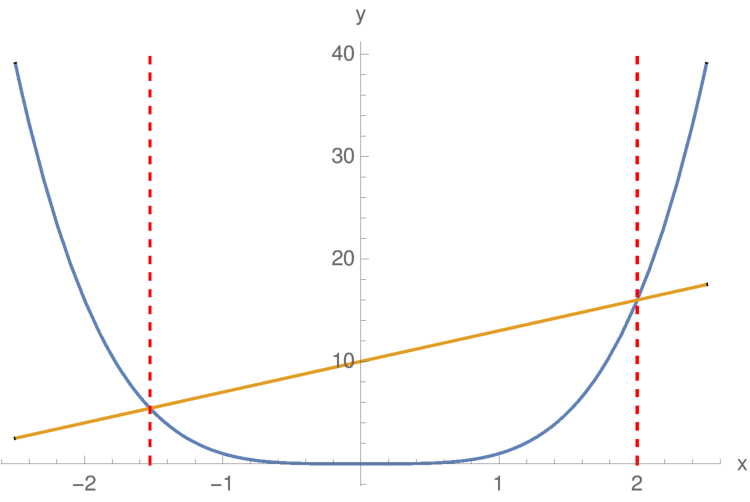
\includegraphics[width=0.9\linewidth]{convex_function.pdf}
\caption{\label{fig:convex}The function $f(x)=x^4$ is plotted in blue. The convexity of this function can be seen by picking any two values of $x$ and noting that $f(x)$ will always lie below or on the chord connecting these two points.} 
\end{figure}

\subsection{Disciplined convex programming}
\noindent In order to solve convex optimisation problems, we used \texttt{cvxpy}, a symbolic programming module for Python \cite{cvxpy}. It uses a set of rules, called \textit{disciplined convex programming} (DCP), to determine whether a function is convex. This is implemented using predefined classes containing functions with their curvature and sign, and using general composition theorems from convex analysis \cite{dcp}. If DCP rules can be applied then interior point methods guarantee an optimal solution. 
%Interior point methods work by applying Newton's algorithm to sequences of equally constrained problems. Is it right that Newton's method is used???
 The algorithm works by picking a step and direction to travel in the interior of the feasible convex set, such that the solution progresses towards optimality, for more details on barrier methods and primal-dual methods see \citep[p.561]{cvxpybook}.
 
\section{Example 1: water-filling}
 
\noindent{}One of the simplest problems to solve in communications with convex optimisation is the classic \textit{water-filling} problem.  Here a total power $P$ is to be assigned to $n$ different communications channels, with the objective of maximising the total communication rate.  By Shannon's theorem \citep[p.245]{cvxpybook}, an upper bound for the rate is given by $\log(1+x_i/\alpha_i)$, where $x_i$ be the power allocated to the $i$th channel and $\alpha_i$ is the noise power in that channel. This can be written as $\log(\alpha_i+x_i)-\log(\alpha_i)$ and the constants $\log(\alpha_i)$ disregarded for the purposes of maximization, and thus the communication rate $r_i$ of the $i$th channel is given by
 \begin{align}
  r_i = \log(x_i+\alpha_i).
 \end{align}
This can be seen in Figure~\ref{fig:waterfilling} as being analogous to filling an uneven basin to a constant level (hence the name \textit{water-filling}).
 
Noting that all power allocations must be non-negative, the optimisation problem can therefore be formulated as,
 \begin{align}
\text{minimise} \quad  -&\sum_{i=1}^{n} \log(x_i+\alpha_i) \nonumber \\
\text{subject to} \quad &x_i \geqslant 0, \quad \forall i \nonumber \\
&\sum_{i=1}^{n}x_i = P.
 \end{align}
This is a convex problem since $-\log(x_i+\alpha_i)$ has positive curvature within the domain $x_i \geqslant 0$, and all the constraints are affine and therefore convex.

\subsection{Implementation}
\noindent We decided to solve the water-filling problem using \texttt{cvxpy} with $n=3$ channels and $(\alpha_1,\alpha_2,\alpha_3) = (0.8,1.0,1.2)$.  For simplicity we chose a dimensionless total power $P=1$.  Using these parameters, the maximum communication rate is, $\sum_{i=1}^{n}r_i = 0.863$, which is achieved with power allocations $(x_1,x_2,x_3) = (8/15,5/15,2/15)$.  This is the solution shown in Figure~\ref{fig:waterfilling}.

\subsection{Example Code}
\noindent To indicate the brevity of code implementation in \texttt{cvxpy} we show a minimal working example below with the parameters chosen above.  With an ordinary commercially available laptop, the time taken to execute the code was around 4ms.
\lstinputlisting[language=Python,mathescape=true,inputencoding=utf8,literate={α}{$\alpha$}1 ]{waterfilling.py}

\begin{figure}[H]
\centering
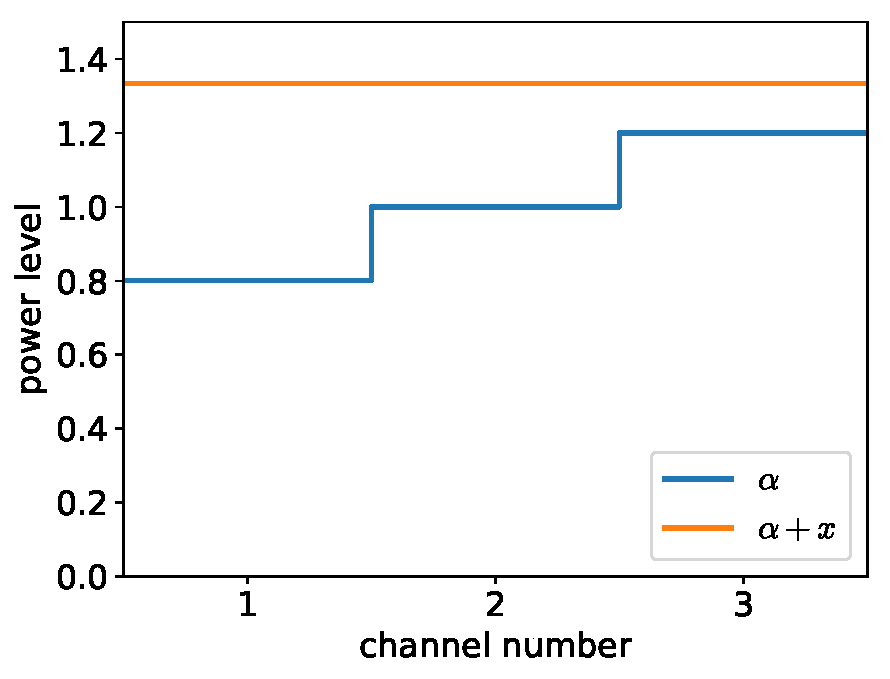
\includegraphics[width=1.0\linewidth]{water_filling_plot.pdf}
\caption{The optimal solution to the water-filling problem allocates the greatest amount of power, $x$, to the channel with the lowest noise power, $\alpha$.}
\label{fig:waterfilling}
\end{figure}

\section{Example 2: power minimisation in communications}
\noindent To demonstrate the applicability of \texttt{cvxpy} to  a real-world example, we consider a system of $n$ transmitters each of power $p_k$, ($k=1,2,...,n$) and $m$ receivers, all in two-dimensional Euclidean space \cite{shannon1949}. At receiver $i$ there is a power $S_i$ of the desired signal, and an interference power $I_i$ from undesired signals, and a background noise $\sigma$. In this problem we are constrained to having a specified minimum signal-to-interference-plus-noise ratio (SINR or $\gamma$) at each receiver
\begin{equation}
\gamma_i =\frac{S_i}{I_i+\sigma}.
\end{equation} 

How can we minimise the total power consumption, $P$, of transmitters, yet achieve this minimum SINR, $\gamma_0$, for all $i$ receivers ($i = 1,2,...,m$)? This question is relevant to telecom companies who want to offer a service at a minimum quality standard. We formulate the problem with a given square path-gain matrix, $G$, background noise level vector $\sigma$, a maximum power constraint $P_{\text{max}}$ of each transmitter and the fact that all transmitters must be supplied with positive power:
\begin{align*}
&\underset{p}{\text{minimise}} \quad &&\sum_k p_k\\
&\text{subject to} \quad &&p_k \leqslant P_{\max}\\
& \quad &&p_k \geqslant 0\\
& \quad &&\gamma_i \geqslant \gamma_0.&&
\end{align*}

Supposing that we want to receive a signal at receiver $i$ from transmitter $k$, we define the recipient matrix, $\Delta$, as
\begin{align*}
\Delta_{ij} = \begin{cases}
1, \quad j=k\\
0, \quad j\neq k
\end{cases},
\end{align*}
and our signal potential matrix $\hat{S}$ as $\hat{S} = G\Delta$.  This means that signal received at transmitter $i$ is $S_i = \hat{S}_{ik}p_k = G_{ik}p_k$.
% The desired signal for receiver $i$ is $S_i = G_{ik}p_k$, 
While the interference potential matrix is defined as $\hat{I} = G-\hat{S}$, giving the interference at $i$ is $I_i = (\hat{I}*p)_i = \sum_{j\neq k}G_{ij}p_j$. We must note that DCP does not allow division of the optimisation variable $p_i$, as it cannot guarantee curvature, so  
\begin{equation*}
  \gamma_i \geqslant \gamma_0\Longleftrightarrow  \frac{S_i}{\sigma_i + I_i} = \frac{\hat{S}_{ik}p_k}{\sigma_i+(\hat{I}*p)_i} \geqslant \gamma_0, \quad \forall i
\end{equation*}
is rearranged to
\begin{equation*}
\hat{S}_{ik}p_k-\gamma_0(\sigma_i + (\hat{I}*p)_i)\geqslant 0, \quad \forall i,
\end{equation*} 
which is affine, and hence a DCP function.

\subsection{Path gain}
%\noindent The path gain $G_{ij}$ represents the proportion of power that reaches receiver $i$ from transmitter $j$. Supposing that the desired signal to receiver $i$ is from transmitter $k$, the power received is,
%\begin{equation}
%p_{ik}^{\text{rec}} = G_{ik}p_k.
%\end{equation}
%Denoting the SINR at $i$ by $\gamma_i$, we have
%\begin{equation}
%\gamma_i = \frac{G_{ik}p_k}{\sigma_i+\sum_{j\neq k}G_{ij}p_j}
%=\frac{S_i}{\sigma_i+I_i}.
%\end{equation}
\noindent In a physical context, the path gain from transmitter $j$ to receiver $i$, as shown in Fig.~\ref{fig:pathgain}, will depend on the distance $d_{ij}$ between them. Assuming isotropic propagation from each transmitter, the fraction of power from $j$ that reaches $i$ is:
\begin{equation}
G_{ij} = A_i/d_{ij}^\alpha
\end{equation}
where $\alpha$ is the pathloss coefficient and $k$ is a proportionality constant specific to the receiver $i$.  For free space $\alpha = 2$, while in urban environments $\alpha \sim 3.5$ \cite{hata1980}. Further physical complexities, such as the stochastic effects from Rayleigh fading can be easily incorporated, whilst remaining within the DCP framework.

\begin{figure}[H]
\centering
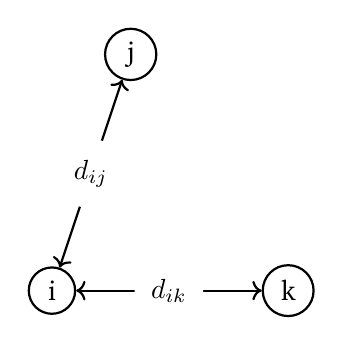
\begin{tikzpicture}
\begin{scope}[every node/.style={circle,thick,draw}]
    \node (A) at (0,0) {i};
    \node (B) at (1,3) {j};
    \node (C) at (3,0) {k};
\end{scope}
\begin{scope}[
	every node/.style={fill=white,circle},
    every edge/.style={draw=black, thick}]
    \path [<->] (A) edge node {$d_{ik}$} (C);
    \path [<->] (B) edge node {$d_{ij}$} (A);
    %\path [<->] (C) edge node {$1$} (B);
\end{scope}
\end{tikzpicture}
\caption{\label{fig:pathgain}Path lengths between receiver $i$ and transmitters $j$ and $k$.}
\end{figure}

\subsection{Implementation}
\noindent For ease of terminology, we will make a few simplifying assumptions.  First, we set the number of transmitters equal to the number of receivers, so $n=m$.  We also pair receiver $i$ to transmitter $k$ such that $i=k$.  This means that the recipient matrix $\Delta$ is the $n\times n$ identity matrix.

All the parameters we will take as dimensionless to give simple numbers to work with.  The maximum available power, $P_{\text{max}}$ is set to 1.  We have chosen the background noise vector $\sigma$ as constant for each receiver, with $\sigma_i = 5$.  Similarly, the receiver coefficient $A$ was set to $0.025$ for each receiver. \\ 

To generate the gain matrix $G$, we randomly sample distances from a given distribution.  For paired transmitters and receivers ($k=i$), we sample $d$ from a scaled $\beta(2,2)$ distribution, such that $d_{ii} \sim 0.2\times\text{Beta}(2,2)$.  For unpaired transmitters and receivers ($k\neq i$), we sample $d$ from a uniform distribution, such that $d_{ik} \sim \text{Uniform}(0,1)$.  This is illustrated in Figure~\ref{fig:dist}.

\begin{figure}[h!]
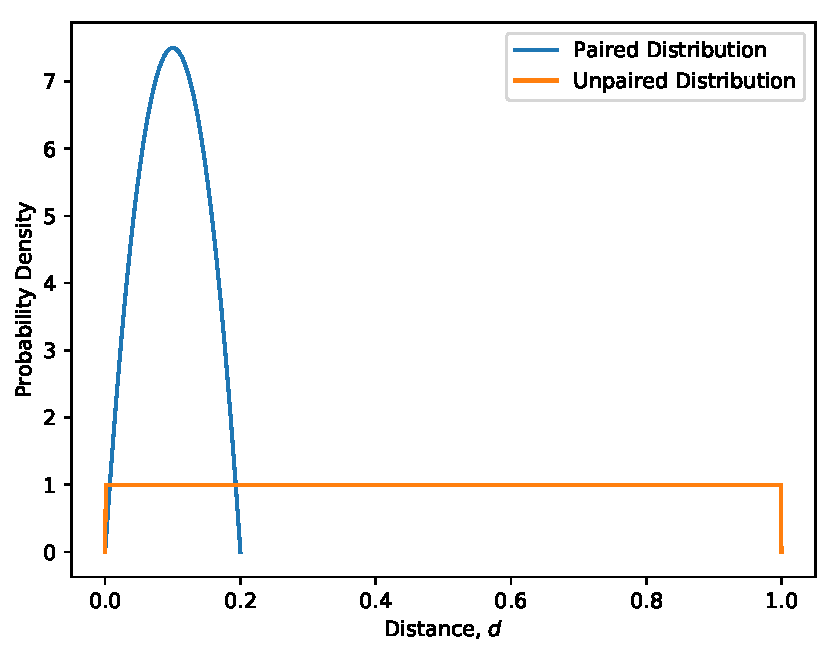
\includegraphics[width=0.9\linewidth]{distance_distributions.pdf}
\caption{\label{fig:dist}The distance between unpaired transmitters and receivers has a higher variance than paired ones, but on average the unpaired distances are expected to be greater.} 
\end{figure}

\subsection{Example code}
\noindent For the random seed of 100 given, the optimal total power consumption is $P = 0.381$, with $p_1,p_2,p_3 = (0.139, 0.072, 0.169)$.  The time taken to find this solution was around 3ms.  Around 70\% of the simulations with these parameters have a feasible solution, with an average optimal power consumption of $P\sim0.4$.

\lstinputlisting[language=Python,mathescape=true,inputencoding=utf8,literate={Δ}{$\Delta$}1 {σ}{$\sigma$}1 {γ}{$\gamma$}1 {∈}{$\in$}1 ]{minimisePgivenSINR.py}

\section{Outlook}
\noindent The authors hope that this article shows the utility of \texttt{cvxpy} for simple `toy' problems of real-world relevance. $\texttt{cvxpy}$ can handle problems with up to $\sim 10^3$ transmitters, however this takes $\sim 10^{4}-10^{5}\text{ms}$ to run, hence for large real-world problems a faster implementation would likely be required (e.g., a \cpp-based library). However, there is obviously a trade-off in terms of ease of understanding with these packages.

We believe that $\texttt{cvxpy}$ is an invaluable resource for researchers wanting to test the applicability of convex optimisation in new fields. The module could also be easily incorporated into a course on optimisation, providing students with an accessible environment to practise techniques for convex optimisation. Full code for other communication examples can be found at \url{https://github.com/cvxgrp/cvxpy/\\tree/master/examples/communications}.

%While all problems that can be written in DCP are convex, not all convex problems of interest can be written in DCP.  Over time, the library of available DCP functions in \texttt{cvxpy} has grown, increasing the scope of convex optimisation problems that \texttt{cvxpy} can solve.  This expansion of scope of \texttt{cvxpy} is ongoing, with version 1.0 under development and expected in the near future.

%\section{Further Work}
%While many problems are convex, others fall into a similar category of being \textit{quasi-convex}.  A quasi-convex function $f$ is one for which $\textbf{dom} f$ and every sublevel set of $f$ is convex.  An example of this is shown in Figure [?].  Quasi-convex problems cannot be solved directly using convex optimisation solvers, however the feasibility of a sublevel set can be checked.  This feasibility check can be used as a bisection method to find the solution.  A more thorough discussion of quasi-convex problems can be found in \cite{cvxpybook}chapter?.

\subsection*{Acknowledgements}
\noindent{}We would like to thank S.~Johnson and S.~Diamond for helpful discussions. 

\subsection*{Author Biography}
\noindent{}Robert Gowers, Sami Al-Izzi, Timothy Pollington, and Roger Hill are PhD students in the Mathematics for Real-World Systems CDT at the University of Warwick.  Keith Briggs is a esearch mathematician at BT.

\vspace{0.2cm}
%\section{Links \& references}
\bibliography{articleBib} 
\bibliographystyle{plain}

%\item DCP analyser http://dcp.stanford.edu/analyzer
% -----
\end{document}
